%Template from a website I found, edited to be in Germanglisch
%=========================================================
%------------GOD--LEFT--US
%=========================================================
\documentclass[12pt]{exam}
%=========================================================
%------------Clearence
%=========================================================
\usepackage[T1]{fontenc}%Codificação
\usepackage[utf8]{inputenc}%Inclui palavras com acento
\usepackage[section]{placeins}
\usepackage[brazil]{babel} %Traduz para o português
\usepackage[top=2cm,left=1cm,right=1.5cm,bottom=2cm]{geometry}%margens
\usepackage{amsmath,amssymb}%Expressoes matemáticas e símbolos
\RequirePackage{amssymb, amsfonts, amsmath, latexsym, verbatim, xspace, setspace}
\usepackage{multicol}% Múltiplas colunas
\usepackage{multirow}% permite mesclar células de modo horizontal
\usepackage{array}%para tabelas
\usepackage{ragged2e}%alinhamento
\usepackage{graphicx}%Para inserir imagens
\usepackage{pdflscape}%Permite mudar a orientacao da pagina
\usepackage{epstopdf} %converte figs eps em figs pdf
\usepackage{booktabs}%tabelas
\usepackage{pdfpages}%Permite incluir arquivos pdf
\usepackage[sort&compress,square,comma, authoryear]{natbib}%Reference
\usepackage[colorlinks=true,urlcolor=magenta,citecolor=red,linkcolor=blue,bookmarks=true]{hyperref}%Links
\usepackage{enumerate}
\usepackage{enumitem}
%---Subitems---
\newlist{partes}{enumerate}{3}
\setlist[partes]{label=(\alph*)}
\newcommand{\parte}{\item}
%---
\newlist{subpartes}{enumerate}{3}
\setlist[subpartes]{label=\roman*)}
\newcommand{\subparte}{\item}
\setlist[enumerate,1]{%(
	leftmargin=*, itemsep=12pt, label={\textbf{\arabic*.)}}}
\newcommand{\dis}{\displaystyle}
\renewcommand*\half{.5}
\newcommand\answerbox{%%
	\fbox{\rule{2in}{0pt}\rule[-0.1ex]{0pt}{4ex}}}
\pointpoints{Punkte}{Punkten}
\hqword{\textcolor{blue}{Frage:}}
\hpword{Wert:}
\hsword{Erhalten:}
\htword{\textcolor{blue}{Total}}
%=========================================================
%------------Header
%=========================================================
\newcommand{\orgao}{Discord Universität München}
\newcommand{\escola}{Elektrotechnik und Informatik}
\newcommand{\disciplina}{Schatungstheorie}
\newcommand{\professor}{Mike Ock}
\newcommand{\data}{\today}
\newcommand{\prova}{1. Prüfung GOP}
\newcommand{\tempo}{15 Minuten}
\newcommand{\aluno}{\bf Name:}
\newcommand{\nota}{NOTE:}
%=========================================================
%-----------Weird stuff
%=========================================================
\pagestyle{headandfoot}%{head}%empty
\firstpageheader{}{}{}
\runningheader{\prova}{}{\data}
\runningheadrule
\firstpagefooter{}{}{}
\runningfooter{}{Viel Glück!}{Seite. \thepage\ von \numpages}
\runningfootrule
%========================================================
\begin{document}
	\fontsize{14}{14}\selectfont
	%========================================================
	%-------------------Main Page
	%========================================================
	\begin{tabular*}{\textwidth}{l @{\extracolsep{\fill}}l @{\extracolsep{6pt}}l}

		\textbf{\orgao} & \textbf{Note:} & {\answerbox}\\

		\textbf{\escola} &\textbf{Fach:}&\textbf{\disciplina}\\
		%-------------------Discipline and Proffesor Name
		\textbf{Professor: \professor}  & {\bf Matr Num.}:&\textbf{\hrulefill}\\[8pt]
		%-------------------
		%\Large{\aluno\textbf{\hrulefill}}& {\bf Turma}:&\textbf{\hrulefill}
		\multicolumn{3}{l}{\Large{\aluno \textbf{\hrulefill}}}\\
	\end{tabular*}
	%--------------------CENTRAL LINE
	\begin{center}
		\rule[1ex]{\textwidth}{1pt}
		{\LARGE{\prova}}\\
		Dauer: \tempo \hspace{9cm}Datum:\hspace{1cm}/\hspace{1cm}/\hspace{1cm}\\
		\rule[2ex]{\textwidth}{1pt}
	\end{center}
	%=========================================================
	%-------------------Reference(S)
	%=========================================================
	\noindent
	Diese klasur erfasst \numpages\ seite(n), instgesamt \numquestions\ Aufgaben, insgesamt \numpoints\ punkte.
	%=========================================================
	%-------------------Point Table
	%=========================================================
	\begin{center}
		\textbf{Tabelle (NUR VON PRÜFER ZU ERFÜLLEN)}\\
		\addpoints
		\gradetable[h][questions]
	\end{center}
	
	\noindent
	\rule[1ex]{\textwidth}{1pt}
	%--------------------something related to table
	\begin{questions}
		%=========================================================
		%-------------------Questions
		%=========================================================
		\question[\half]Aufgabe 1: Geben sie eine Ersatzschaltbild fur Tesla Roadster Motor, nur aus Zweitoren bestehnd. (Gegebene Platz ist genügend.)
\makeemptybox{2in}
		
		\question[\half]Aufgabe 2: Überprüfen sie mithilfe der vorliegenden 40x20 Betriebsmatrix das abgebildete 20-Tor auf strenge Linearität (Abbildung auf nächste Seite.)
\makeemptybox{2in}
		\begin{figure}[!htbp]
			\centering
			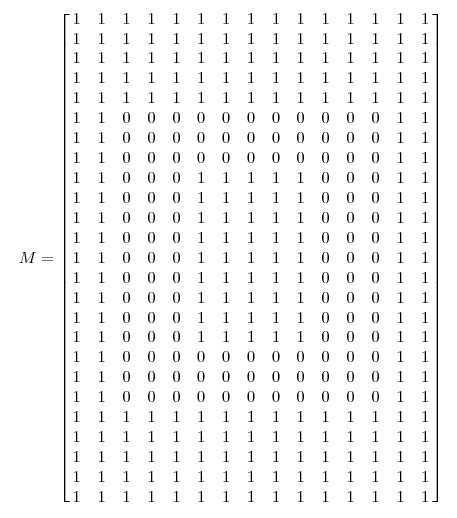
\includegraphics[width=0.7\linewidth]{matrix}
		
			
		\end{figure}
		\FloatBarrier

		%---------------------------------------------------------
		\question[5] Aufgabe 3:
		Stellen Sie sich vor, Sie sind ein Ingenieur von der CERN.  Entwerfen Sie das CERN Aufbau von Grund auf neu und effizienter. Dazu verwenden Sie die Allgemeine Analyseverfahren aus Kap.7 aus Skriptum!
\makeemptybox{2in}
		\addpoints
		%----------------------------------------------------------
		\question[90]Aufgabe 4:
		Stellen sie sich vor sie gingen zu Media Markt, in welcher Abteilung findet man im Normalfall die Nullatoren, Noratoren, Nullore und idealen Übertragern?
		\\
		%----------------------------------------------------------
		\question[1] Ihre kollegin aus Nord Korea hat ihre schaltung nachgebaut und ein messung wo $u^Ti=5$ ist, erhalten. Was passiert zu sie?
		
		\begin{choices}
			\choice Sie ist getötet.
			\choice Sie hat ein Gyrator gegessen.
			\choice She defected to South Korea.
			\choice [REDACTED]
		\end{choices}
		%----------------------------------------------------------
		\question[1] Stellen sie die Hybridmatrix des 80 Tors auf
		\\
		\begin{figure}[!htbp]
			\centering
			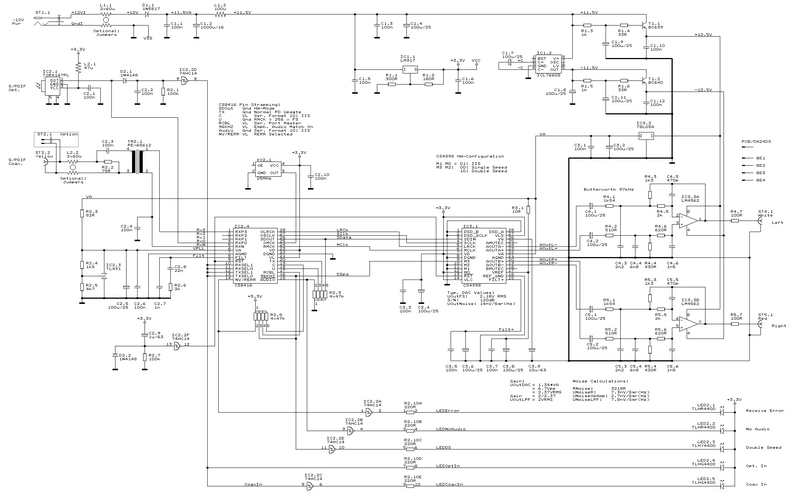
\includegraphics[width=0.7\linewidth]{unknown}
			\caption{Ein 80-Tor}
			\label{fig:unknown}
		\end{figure}
		
		
		%----------------------------------------------------------
		\question[1] *Geben sie zu vorliegendem ESB die Spannung u1 (unten rechts) in abhängigkeit von u234 (oben links) an.
\makeemptybox{3in}
		
		%-----------------------------------------------------------

		\addpoints
		%---------------------------------------------------------------
		\question[2]Geben Sie eine Schaltung, mit der die Anzahl der im Februar exmatrikulierten Studenten bestimmt werden soll. Geben sie an warum sie übertaktet werden muss.
		\makeemptybox{2in}
		%---------------------------------------------------------------
		\newpage
		
		
		%=========================================================
		%-------------------End of Document EOF
		%=========================================================
	\end{questions}
	%===========================================================
	%          BIBLIOGRAPHY
	%===========================================================

\end{document}